% Slide bảo vệ giữa kỳ, phần B (Nguyễn Ngọc Bích).
% Biên dịch bằng XeLaTeX (Overleaf: Menu > Compiler > XeLaTeX). Cùng mẫu với slides_a.tex.
\documentclass[aspectratio=169,11pt]{beamer}

\usepackage{fontspec}
\setmainfont{texgyreheros}[Extension=.otf,UprightFont=*-regular,BoldFont=*-bold,ItalicFont=*-italic,BoldItalicFont=*-bolditalic]
\setsansfont{texgyreheros}[Extension=.otf,UprightFont=*-regular,BoldFont=*-bold,ItalicFont=*-italic,BoldItalicFont=*-bolditalic]
\setmonofont{texgyrecursor}[Extension=.otf,UprightFont=*-regular,BoldFont=*-bold,ItalicFont=*-italic,BoldItalicFont=*-bolditalic]
\usepackage[vietnamese]{babel}
\usepackage{tikz}
\usetikzlibrary{arrows.meta,positioning,calc}
\usepackage{tabularx}
\usepackage{booktabs}
\usepackage{colortbl}
\usepackage{array}

% ---- Màu: giống slides_a.tex ----
\definecolor{accent}{RGB}{68,114,196}
\definecolor{accentlight}{RGB}{234,240,250}
\definecolor{accentdark}{RGB}{38,62,110}
\definecolor{ink}{RGB}{38,42,52}
\definecolor{muted}{RGB}{110,116,128}
\definecolor{warn}{RGB}{196,80,90}

\setbeamercolor{normal text}{fg=ink,bg=white}
\setbeamercolor{structure}{fg=accent}
\setbeamercolor{frametitle}{fg=accentdark,bg=white}
\setbeamercolor{itemize item}{fg=accent}
\setbeamercolor{itemize subitem}{fg=accent}
\setbeamercolor{block title}{fg=white,bg=accent}
\setbeamercolor{block body}{fg=ink,bg=accentlight}
\setbeamertemplate{navigation symbols}{}
\setbeamertemplate{itemize item}[square]
\setbeamertemplate{itemize subitem}[circle]
\setbeamerfont{itemize/enumerate body}{size=\normalsize}
\setbeamerfont{itemize/enumerate subbody}{size=\small}
\setbeamertemplate{blocks}[rounded][shadow=false]

\setbeamertemplate{frametitle}{%
  \vskip 3mm
  \usebeamercolor[fg]{frametitle}\usebeamerfont{frametitle}\bfseries\Large\insertframetitle\par
  \vskip 1.2mm
  {\color{accent}\hrule height 1.2pt}
}
\setbeamertemplate{footline}{%
  \hbox to \paperwidth{%
    \hspace{8mm}\color{muted}\scriptsize Nguyễn Ngọc Bích \textbar\ Phát hiện biển số xe và tách ký tự bằng xử lý ảnh cổ điển%
    \hfill\insertframenumber\,/\,\inserttotalframenumber\hspace{8mm}}
  \vskip 4mm}
\setbeamersize{text margin left=9mm,text margin right=9mm}

\newcommand{\code}[1]{{\footnotesize\ttfamily #1}}
\newcommand{\acc}[1]{\textcolor{accent}{\textbf{#1}}}
\newcommand{\hl}[1]{\textcolor{accentdark}{\textbf{#1}}}

\renewcommand{\arraystretch}{1.18}
\newcommand{\hd}[1]{\cellcolor{accent}\textcolor{white}{\bfseries #1}}
\newcolumntype{C}{>{\centering\arraybackslash}X}
\newcolumntype{Y}{>{\raggedright\arraybackslash}X}

\title{Phát hiện biển số xe và tách ký tự\\bằng xử lý ảnh cổ điển}
\subtitle{Báo cáo giữa kỳ, phần B: hệ màu, nhị phân hóa, tách ký tự}
\author{Bùi Thuỳ Châu Anh (24001963)\and Nguyễn Ngọc Bích (24001977)}
\date{MAT3562E Computer Vision, HK1 2026--2027}

\begin{document}

% ============ 1. Tiêu đề ============
\begin{frame}[plain]
  \begin{tikzpicture}[remember picture,overlay]
    \fill[accent] (current page.north west) rectangle ([yshift=-4.2cm]current page.north east);
    \node[anchor=north west,xshift=9mm,yshift=-7mm,text=white,align=left] at (current page.north west)
      {\fontsize{9}{11}\selectfont\bfseries TRƯỜNG ĐẠI HỌC KHOA HỌC TỰ NHIÊN, ĐHQGHN};
    \node[anchor=north east,xshift=-9mm,yshift=-5mm,fill=white,rounded corners=3pt,inner sep=2.5mm] at (current page.north east)
      {
\includegraphics[height=2.3cm]{figures/HUS.png}};
    \node[anchor=south west,xshift=9mm,yshift=-4.2cm+4mm,text=white,align=left,text width=0.72\paperwidth] at (current page.north west)
      {\fontsize{22}{26}\selectfont\bfseries Phát hiện biển số xe và tách ký tự bằng xử lý ảnh cổ điển};
  \end{tikzpicture}
  \vspace{3.55cm}
  \begin{flushleft}
    {\large\bfseries\color{accentdark} Báo cáo giữa kỳ: phần B}\\[1mm]
    {\color{muted}Phân tích hệ màu, nhị phân hóa và tách ký tự}\\[5mm]
    \small
    \begin{tabular}{@{}l@{\hspace{6mm}}l@{}}
      \hl{Nhóm thực hiện} & Bùi Thuỳ Châu Anh (24001963), Nguyễn Ngọc Bích (24001977)\\
      \hl{Môn học} & MAT3562E Computer Vision, HK1 2026--2027\\
      \hl{Giảng viên} & TS. Cao Văn Chung\\
    \end{tabular}
  \end{flushleft}
\end{frame}

% ============ 2. Vị trí phần B + độ đo ============
\begin{frame}{Phần B trong pipeline và cách đo}
  \centering
  \begin{tikzpicture}[
    node distance=6mm,
    boxA/.style={draw=muted,dashed,thick,rounded corners=3pt,align=center,minimum height=15mm,text width=27mm,font=\footnotesize,text=muted},
    boxB/.style={draw=accent,fill=accentlight,thick,rounded corners=3pt,align=center,minimum height=15mm,text width=27mm,font=\footnotesize},
    arr/.style={-{Stealth[length=2.4mm]},thick,color=accentdark}]
    \node[boxA] (a) {\textbf{Phần A}\\định vị, nắn về\\ảnh $220\times70$};
    \node[boxB,right=of a] (bin) {\textbf{Nhị phân hóa}\\Otsu / adaptive\\(E5)};
    \node[boxB,right=of bin] (seg) {\textbf{Tách ký tự}\\CCA / projection\\(E6)};
    \node[boxB,right=of seg] (out) {Danh sách\\hộp ký tự\\trái $\to$ phải};
    \draw[arr] (a)--(bin); \draw[arr] (bin)--(seg); \draw[arr] (seg)--(out);
  \end{tikzpicture}
  \vspace{3mm}

  \begin{columns}[T]
    \column{0.52\textwidth}
    \begin{itemize}
      \item Ngoài ra: \acc{E1} phân tích hệ màu, \acc{E0} khung \code{run\_all}, công cụ gán nhãn ký tự, \acc{E8} ảnh biển VN.
      \item Khuôn 7 vị trí chuẩn của biển $440\times140$ mm, quy về ảnh $220\times70$.
      \item Crop \code{gt} (quad thật): đo riêng bộ tách. Crop \code{pred}: cả pipeline.
    \end{itemize}
    \column{0.45\textwidth}
    \begin{block}{Độ đo}
      \small
      \code{count\_match}: đủ 7 hộp.\\
      \code{pos0}, \code{pos1-6}: hộp trúng khuôn vị trí.\\
      \code{all\_correct}: đủ 7 hộp \emph{và} cả 7 vị trí trúng.
    \end{block}
  \end{columns}
\end{frame}

% ============ 3. E1 ============
\begin{frame}{E1: kênh màu nào tách biển khỏi nền tốt nhất?}
  \begin{columns}[T]
    \column{0.36\textwidth}
    \begin{itemize}
      \item Histogram 64 bin trong bbox biển ($p$) và phần còn lại ($q$), tune $n=198$.
      \item Khoảng cách Bhattacharyya
      \[D=\sqrt{1-\textstyle\sum_i\sqrt{p_iq_i}}\]
      \item \hl{b (Lab) 0.657, H (HSV) 0.654} tốt nhất; S 0.513; xám chỉ \hl{0.472}.
      \item Biển CCPD nền xanh: dồn vào $H\approx100$--$120$, $b<128$.
    \end{itemize}
    \column{0.62\textwidth}
    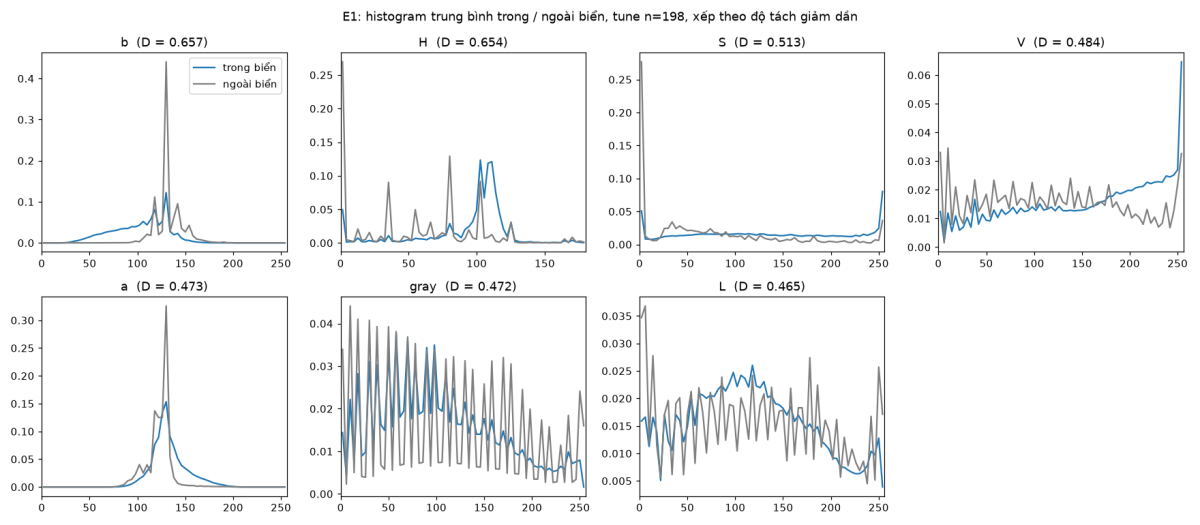
\includegraphics[width=\linewidth]{figures/b_e1_hist.png}\\[-1mm]
    {\footnotesize\color{muted} Xanh: trong biển, xám: ngoài biển. Thứ hạng 3 kênh đầu không đổi với 32 và 128 bin.}
    \vspace{2mm}

    {\small Hệ quả: định vị đang dùng ảnh xám. Nguồn ứng viên theo màu là hướng bổ sung (chưa thử), nhưng \hl{chỉ đúng với biển nền xanh}, không dùng được cho biển VN nền trắng/vàng.}
  \end{columns}
\end{frame}

% ============ 4. Nhị phân hóa: phương pháp ============
\begin{frame}{Nhị phân hóa: Otsu và adaptive}
  \begin{columns}[T]
    \column{0.49\textwidth}
    {\bfseries\color{accentdark}Otsu: một ngưỡng cho cả biển}
    \[t^{*}=\arg\max_{t}\;\omega_0\,\omega_1\,(\mu_0-\mu_1)^2\]
    \begin{itemize}
      \item Cực đại phương sai giữa hai lớp (nền, chữ).
      \item Hợp khi biển sáng đều, histogram hai đỉnh.
    \end{itemize}
    \vspace{2mm}
    {\bfseries\color{accentdark}Adaptive: ngưỡng riêng cho từng pixel}
    \[T(x,y)=m_G(x,y)-C,\quad 25\times25,\; C=7\]
    \begin{itemize}
      \item Chịu được bóng đổ, chói một bên.
    \end{itemize}
    \column{0.48\textwidth}
    \begin{block}{Lỗi gặp khi cài adaptive}
      \small Biển xanh chữ trắng: nền phẳng thành trắng, ký tự chỉ còn \hl{viền rỗng}.\\[1mm]
      Sửa: dùng Otsu để đoán cực tính (chữ sáng thì đảo ảnh), rồi \code{THRESH\_BINARY\_INV}. Có test đơn vị kiểm tra nền phẳng phải đen.
    \end{block}
    \vspace{2mm}
    \begin{itemize}
      \item Sau đó: đảm bảo chữ trắng (\code{ensure\_text\_white}), mở hình thái $2\times2$ xóa chấm nhiễu.
    \end{itemize}
  \end{columns}
\end{frame}

% ============ 5. E5 kết quả ============
\begin{frame}{E5: Otsu và adaptive cho kết quả tương đương}
  \begin{columns}[T]
    \column{0.45\textwidth}
    {\small\bfseries Test, crop \code{gt}, tách bằng CCA}\\[1mm]
    \small
    \setlength{\tabcolsep}{3pt}\begin{tabularx}{\linewidth}{lcCC}
      \rowcolor{accent}\hd{Nhóm} & \hd{$n$} & \hd{Otsu} & \hd{Adaptive}\\
      base & 350 & \textbf{0.666} & 0.611\\
      \rowcolor{accentlight}blur & 28 & \textbf{0.143} & 0.071\\
      challenge & 28 & 0.143 & \textbf{0.214}\\
      \rowcolor{accentlight}db & 28 & \textbf{0.393} & 0.250\\
      tilt & 28 & \textbf{0.286} & 0.214\\
      \rowcolor{accentlight}\textbf{ALL} & 462 & \textbf{0.563} & 0.509\\
    \end{tabularx}
    {\footnotesize\color{muted} Giá trị là \code{all\_correct}.}
    \vspace{1mm}
    \begin{itemize}
      \item Theo cặp: 90 biển chỉ Otsu đúng, 65 biển chỉ adaptive đúng, $p\approx0.054$.
      \item Trên tune thì ngược lại (0.540 so với 0.566) $\Rightarrow$ \hl{coi là hòa}, giữ Otsu.
    \end{itemize}
    \column{0.53\textwidth}
    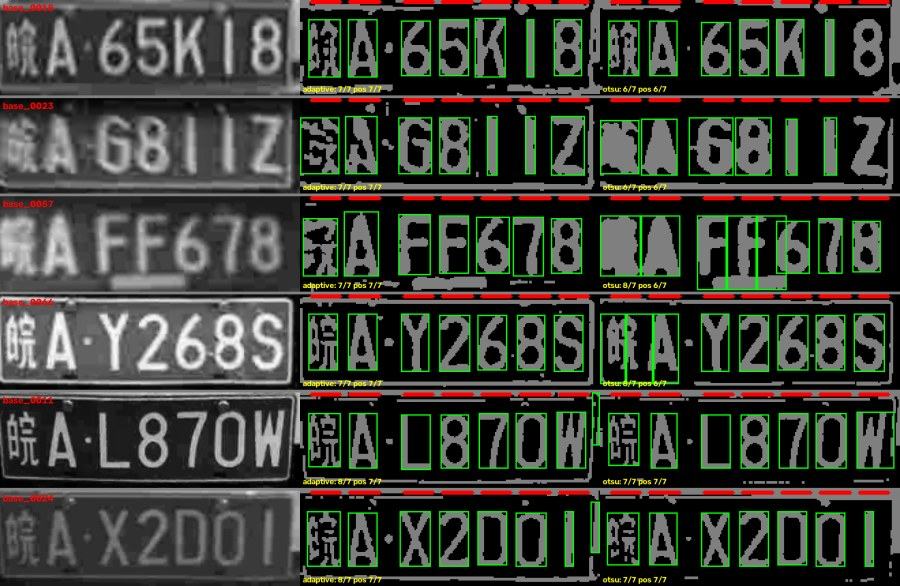
\includegraphics[width=\linewidth]{figures/b_binarize.jpg}\\[-1mm]
    {\footnotesize\color{muted} Ảnh gốc | adaptive | Otsu. Vạch đỏ: khuôn 7 vị trí.}
    \vspace{1mm}

    {\small Hai kiểu lỗi ngược nhau: \hl{Otsu hay làm dính} ký tự (148 biển $\le6$ hộp), \hl{adaptive hay sinh hộp thừa} ở mép viền (85 biển $\ge8$ hộp).}
  \end{columns}
\end{frame}

% ============ 6. Tách ký tự: phương pháp ============
\begin{frame}{Tách ký tự: CCA và projection}
  \begin{columns}[T]
    \column{0.49\textwidth}
    {\bfseries\color{accentdark}CCA (thành phần liên thông)}
    \begin{enumerate}
      \item Bỏ viền (rộng, rỗng), ốc vít (tâm lệch dọc). Khối rộng mà \emph{đặc} thì giữ lại để cắt.
      \item Gộp mảnh chồng nhau theo $x$ (ký tự Hán vỡ nét), gộp mảnh hẹp với mảnh kề.
      \item Lọc chiều cao, tỉ lệ, diện tích.
      \item Hộp rộng $\ge1.7\,w_{\mathrm{med}}$: \hl{cắt đều} thành $\mathrm{round}\big(\tfrac{w+g}{w_{\mathrm{med}}+g}\big)$ phần.
    \end{enumerate}
    \column{0.49\textwidth}
    {\bfseries\color{accentdark}Projection (chiếu theo cột)}
    \begin{enumerate}
      \item Bỏ viền, ốc vít như CCA; tách dòng bằng chiếu ngang.
      \item Profile cột: cột có $\ge10\%$ chiều cao là trắng thì là cột chữ.
      \item Nối dải gần nhau, bỏ dải quá hẹp.
      \item Dải rộng: \hl{cắt tại thung lũng} (cột ít trắng nhất) quanh vị trí dự kiến.
    \end{enumerate}
  \end{columns}
  \vspace{2mm}
  {\small\color{muted} Mọi ngưỡng tính theo tỉ lệ kích thước biển; tham số thí nghiệm lấy từ config.}
\end{frame}

% ============ 7. Tinh chỉnh trên tune ============
\begin{frame}{Tinh chỉnh trên tune: sửa độ đo cho chữ số ``1''}
  \begin{columns}[T]
    \column{0.44\textwidth}
    \begin{itemize}
      \item Số ``1'' rộng $\approx$ 9 px, khuôn 22.5 px $\Rightarrow$ IoU $\approx0.4$ dù nằm đúng giữa khuôn.
      \item Trước khi sửa: chỉ \hl{3/56} vị trí ``1'' được tính đúng, so với 889/994 ký tự khác.
      \item Luật tâm: hộp hẹp ($\le0.6\times$ khuôn) trúng nếu \hl{tâm nằm trong khuôn}.
      \item Issue \#14: ngưỡng mảnh hẹp riêng, cắt có tính khe, lọc mảnh dẹt sau khi gộp.
    \end{itemize}
    \column{0.54\textwidth}
    {\small\bfseries \code{all\_correct}, tune $n=198$, crop \code{gt}}\\[1mm]
    \small
    \setlength{\tabcolsep}{3pt}\begin{tabularx}{\linewidth}{YCC}
      \rowcolor{accent}\hd{Phiên bản} & \hd{Otsu+CCA} & \hd{Otsu+proj.}\\
      Bản đầu & 0.338 & --\\
      \rowcolor{accentlight}Giữ khối đặc để cắt & 0.364 & --\\
      Luật tâm cho ``1'' & 0.515 & 0.566\\
      \rowcolor{accentlight}\textbf{Issue \#14 (chốt)} & 0.540 & \acc{0.596}\\
    \end{tabularx}
    \vspace{2mm}

    {\footnotesize\color{muted} Mỗi bước xuất phát từ đọc ảnh lỗi, không quét lưới. Hằng số chọn trên chính tune nên số tune hơi lạc quan.}
  \end{columns}
\end{frame}

% ============ 8. E6 ============
\begin{frame}{E6: projection tốt hơn CCA, ổn định trên cả hai tập}
  \begin{columns}[T]
    \column{0.47\textwidth}
    {\small\bfseries Test, Otsu, \code{all\_correct}}\\[1mm]
    \small
    \setlength{\tabcolsep}{2.5pt}\begin{tabularx}{\linewidth}{lCCCC}
      \rowcolor{accent}\hd{Nhóm} & \hd{CCA gt} & \hd{proj. gt} & \hd{CCA pred} & \hd{proj. pred}\\
      base & 0.666 & \textbf{0.749} & 0.243 & \textbf{0.277}\\
      \rowcolor{accentlight}blur & 0.143 & \textbf{0.214} & 0.000 & \textbf{0.071}\\
      challenge & 0.143 & \textbf{0.214} & \textbf{0.071} & 0.000\\
      \rowcolor{accentlight}db & \textbf{0.393} & 0.250 & \textbf{0.107} & 0.071\\
      tilt & 0.286 & 0.286 & 0.000 & 0.000\\
      \rowcolor{accentlight}\textbf{ALL} & 0.563 & \acc{0.626} & 0.195 & \acc{0.219}\\
    \end{tabularx}
    \vspace{1mm}
    \begin{itemize}
      \item Theo cặp: 47 / 18 biển, \hl{$p<0.001$}; tune cùng chiều (0.596 / 0.540).
      \item Lợi thế từ \code{count\_match} (0.680 / 0.606): thiếu hộp giảm 148 $\to$ 110 biển.
    \end{itemize}
    \column{0.51\textwidth}
    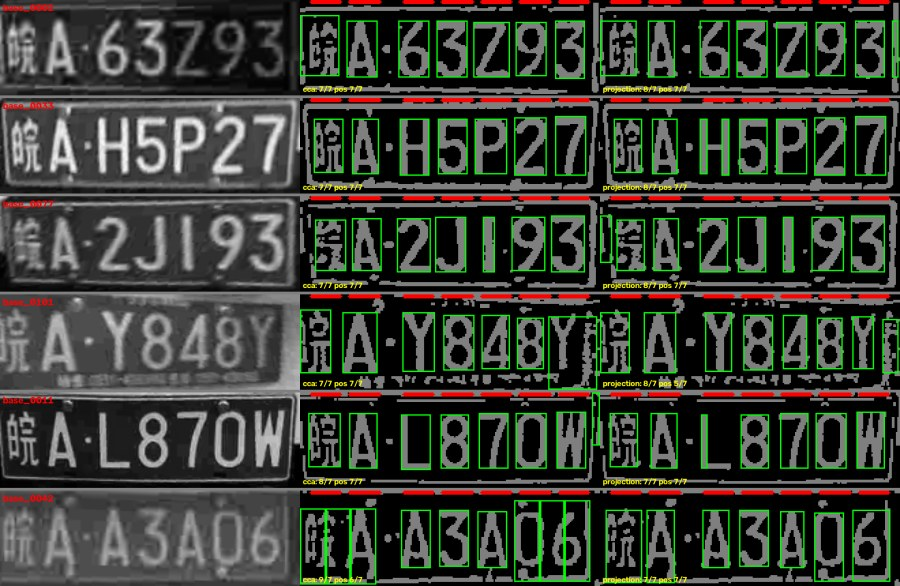
\includegraphics[width=\linewidth]{figures/b_segment.jpg}\\[-1mm]
    {\footnotesize\color{muted} Ảnh gốc | CCA | projection. CCA cắt đều khối ``06'' dính nhiễu thành 3 hộp; projection không bị nhưng hay thừa hộp ở mép, và cắt ``H'' thành hai nét.}
  \end{columns}
\end{frame}

% ============ 9. gt -> pred ============
\begin{frame}{Lỗi tổng thể chủ yếu nằm trước bước tách}
  \begin{columns}[T]
    \column{0.52\textwidth}
    \begin{tikzpicture}[x=4.8cm,y=0.95cm,font=\small]
      \foreach \y/\lab/\v/\t in {3/{proj., crop \code{gt}}/0.626/0.626, 2/{CCA, crop \code{gt}}/0.563/0.563, 1/{proj., crop \code{pred}}/0.219/0.219, 0/{CCA, crop \code{pred}}/0.195/0.195}{
        \node[anchor=east] at (-0.03,\y) {\lab};
        \fill[accent] (0,\y-0.27) rectangle (\v,\y+0.27);
        \node[anchor=west] at (\v+0.02,\y) {\t};
      }
    \end{tikzpicture}\\[1mm]
    {\footnotesize\color{muted} \code{all\_correct} trên test, $n=462$.}
    \column{0.46\textwidth}
    \begin{itemize}
      \item \hl{0.626 $\to$ 0.219} khi thay quad thật bằng quad dự đoán.
      \item 25\% ảnh định vị sai; quad dự đoán lệch trung bình 16 px (E4).
      \item Triage: 64/123 ảnh \code{segment\_count} tách đúng nếu crop bằng quad thật.
      \item Lỗi của chính bộ tách: ký tự Hán \hl{dính chữ ``A''} (6 hộp) và mảnh viền ở mép (8 hộp).
    \end{itemize}
  \end{columns}
  \vspace{2mm}
  \begin{block}{Đánh giá theo hộp gán tay (30 biển test, 210 hộp)}
    \small CCA: P 0.945, R 0.819, F1 0.878 \quad|\quad projection: P 0.962, R 0.838, \hl{F1 0.896} (base: 0.977). P cao hơn R: hộp sinh ra thường ôm đúng ký tự, lỗi chủ yếu là \emph{thiếu} hộp.
  \end{block}
\end{frame}

% ============ 10. E8 + hạn chế ============
\begin{frame}{E8 ảnh biển VN, hạn chế và hướng tiếp theo}
  \begin{columns}[T]
    \column{0.49\textwidth}
    {\bfseries\color{accentdark}E8: biển số Việt Nam}
    \begin{itemize}
      \item Chưa chạy: bộ ảnh tự chụp chưa đưa vào dự án.
      \item Dự đoán khó khăn:
      \begin{itemize}
        \item nền trắng/vàng, chữ đen: bước nhị phân tự đoán cực tính, nhưng SVM và E1 gắn với nền xanh;
        \item biển 2 dòng: \code{split\_lines} mới kiểm bằng ảnh giả;
        \item 7--9 ký tự, không có chữ Hán: khuôn 7 vị trí không áp dụng.
      \end{itemize}
    \end{itemize}
    \column{0.49\textwidth}
    {\bfseries\color{accentdark}Hạn chế}
    \begin{itemize}
      \item Hằng số hình học chọn trên tune.
      \item Khuôn vị trí lệch trái $\approx$ 3 px.
      \item Hộp gán tay chỉ 30 biển (2 biển mỗi nhóm khó).
    \end{itemize}
    {\bfseries\color{accentdark}Hướng tiếp theo}
    \begin{itemize}
      \item Đổi mặc định sang \hl{projection}.
      \item Xử lý riêng ký tự Hán dính ``A''.
      \item Nguồn ứng viên theo màu (từ E1).
    \end{itemize}
  \end{columns}
\end{frame}

% ============ 11. Kết luận chung ============
\begin{frame}{Kết luận chung của nhóm}
  \begin{itemize}
    \item Pipeline cổ điển trên CCPD: định vị \code{edge\_svm} top-1 đúng \acc{75.1\%}, nắn quad, tách projection.
    \item Trên crop thật, bộ tách đúng hết \acc{62.6\%} biển; toàn pipeline chỉ \acc{19.5--21.9\%}.
    \item Nút thắt theo thứ tự ưu tiên:
    \begin{enumerate}
      \item \hl{Sinh ứng viên}: 21\% ảnh không có ứng viên đúng trong top-5 $\to$ thêm ứng viên theo màu, mẫu âm khó cho SVM.
      \item \hl{Nắn}: quad lệch $\approx$ 16 px làm hỏng crop.
      \item \hl{Tách}: ký tự Hán dính ``A'', mảnh viền ở mép.
    \end{enumerate}
    \item Mọi lựa chọn làm trên CCPD (nền xanh, 1 dòng, 7 ký tự); khả năng dùng cho biển VN chưa kiểm chứng.
  \end{itemize}
\end{frame}

% ============ 12. Cảm ơn ============
\begin{frame}[plain]
  \begin{tikzpicture}[remember picture,overlay]
    \fill[accent] (current page.south west) rectangle (current page.north east);
    \node[text=white,align=center,text width=0.8\paperwidth] at (current page.center)
      {{\fontsize{28}{32}\selectfont\bfseries Cảm ơn thầy và các bạn đã lắng nghe}\\[6mm]
       {\large Xin mời thầy và các bạn đặt câu hỏi}};
  \end{tikzpicture}
\end{frame}

\end{document}
